\section{Dataset and Selection Details}
\label{app:ext_data}
\clearpage
\subsection{Float Cited in the Main Text}
The main text cites Table~\ref{tab:cutflow}; it is placed here to keep the main text within its page limit.

\begin{table}[h]
\centering
\resizebox{\ifdim\width>\linewidth\linewidth\else\width\fi}{!}{\begin{tabular}{lrrrr}
\toprule
Requirement & alone & cumulative & down & up \\
\midrule
All candidates & -- & $8{,}556{,}118$ & $5{,}135{,}823$ & $3{,}420{,}295$ \\
$\lnot\texttt{isMuon}$, three tracks & $6{,}311{,}517$ & $6{,}311{,}517$ & $3{,}806{,}297$ & $2{,}505{,}220$ \\
$\texttt{ProbPi}<0.5$, three tracks & $975{,}724$ & $481{,}101$ & $288{,}908$ & $192{,}193$ \\
$\texttt{ProbK}>0.5$, three tracks & $28{,}812$ & $23{,}895$ & $14{,}178$ & $9717$ \\
Mass window $[5100,5600]\,\MeV$ & -- & $19{,}731$ & $11{,}636$ & $8095$ \\
\bottomrule
\end{tabular}}
\caption{Number of candidates passing each requirement alone and after the cumulative selection, in the order of the table, and by magnet polarity. The kaon-identification requirement on the three tracks is by far the most selective.}
\label{tab:cutflow}
\end{table}


\FloatBarrier


\section{Extended Bayesian Analysis}
\label{app:ext_bayes}
\subsection{Model Adequacy: Goodness of Fit and Posterior Predictive Check}
\label{sec:bayes_gof}
\emph{In short: the model does not reach $\chi^2/\mathrm{ndof}\approx1$ ($164.1/88$), mainly because the signal tails are heavier than a Gaussian, but $\Araw$ changes by only $-0.0002$ with a Crystal Ball signal.}
\begin{table}[!t]
\centering
\begin{tabular}{lccc}
\toprule
Model & $\Araw$ & $\chi^2$/ndof & $p$ \\
\midrule
Nominal & $-0.0443$ & $164.1/88$ & $2\times10^{-6}$ \\
Crystal Ball signal & $-0.0445$ & $131.0/86$ & $1\times10^{-3}$ \\
$\mu$, $\sigma$ per charge & $-0.0443$ & $164.2/86$ & $8\times10^{-7}$ \\
Shared bkg.\ shape & $-0.0480$ & $174.1/91$ & $4\times10^{-7}$ \\
Symmetric bkg.\ ($A_b=0$) & $-0.0471$ & $169.8/89$ & $5\times10^{-7}$ \\
Single exponential & $-0.0480$ & $297.7/92$ & $2\times10^{-23}$ \\
\bottomrule
\end{tabular}
\caption{$\Araw$ (posterior median) and goodness of fit of the nominal model (Gaussian signal, double exponential per charge) and of the alternative signal and background models, same data and window.}
\label{tab:gof}
\end{table}

\begin{figure*}[t]
\centering
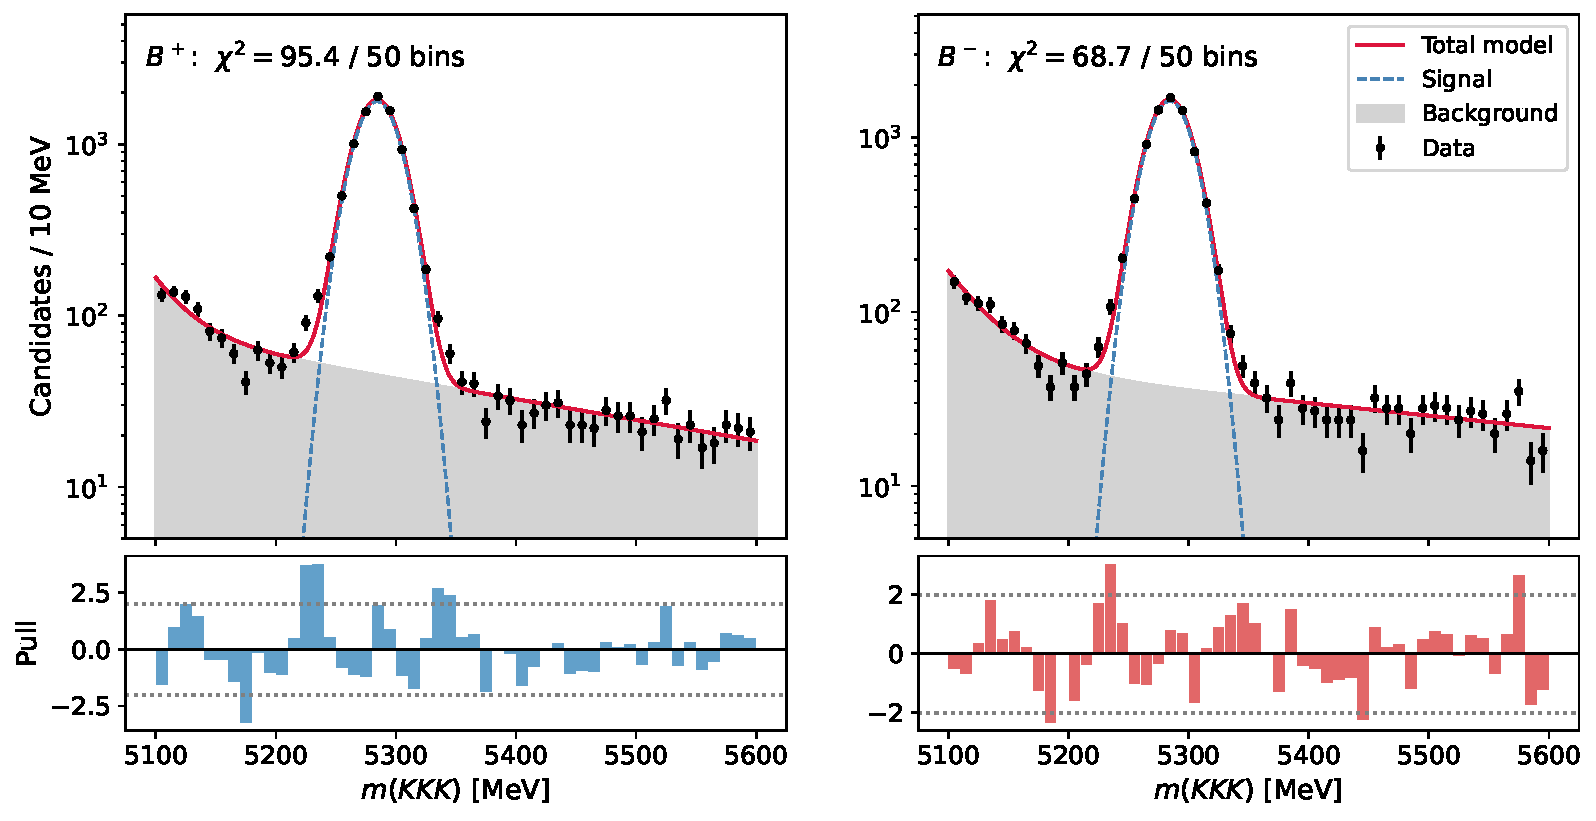
\includegraphics[width=0.95\textwidth]{figures/bayes_nominal_mass_fit.pdf}
\caption{Mass distributions of (a) $B^+$ and (b) $B^-$ candidates with the nominal model (posterior medians, logarithmic scale): total, signal and background components. Bottom: pulls, $(\text{obs}-\text{exp})/\sqrt{\text{exp}}$.}
\label{fig:bayes_fit}
\end{figure*}

A binned comparison of data and posterior-median model ($\chi^2=\sum(\text{obs}-\text{exp})^2/\text{exp}$ over 50 bins of $10\,\MeV$ per charge, $100-12=88$ degrees of freedom) gives $\chi^2=164.1/88$ ($p=1.6\times10^{-6}$), with $95.4$ for $B^+$ and $68.7$ for $B^-$. The largest pulls, in the $B^+$ sample, sit on the two flanks of the peak, about $\pm3\sigma$ from $\mu$ (Fig.~\ref{fig:bayes_fit}): the observed signal shape has heavier tails than a Gaussian. Replacing the Gaussian by a Crystal Ball shape~\cite{skwarnicki}, a Gaussian core with a power-law low-mass tail,
\begin{equation}
S_{\mathrm{CB}}(x)\propto
\begin{cases}
e^{-x^2/2}, & x>-\beta,\\[2pt]
\left(\frac{\kappa}{\beta}\right)^{\kappa} e^{-\beta^2/2}\left(\frac{\kappa}{\beta}-\beta-x\right)^{-\kappa}, & x\leq-\beta,
\end{cases}
\label{eq:cb}
\end{equation}
with $x=(m-\mu)/\sigma$, $\beta$ the point where the tail starts (in units of $\sigma$) and $\kappa$ its power, both free, improves the fit to $\chi^2=131.0/86$ ($p=1.3\times10^{-3}$, $\beta=1.71$, $\kappa=35$) but moves $\Araw$ by only $-0.0002$ (Table~\ref{tab:gof}). The asymmetry does not depend on the signal shape even though none of the models reaches $\chi^2/\text{ndof}\approx1$. The Gaussian is nevertheless kept as the nominal signal model, common to the two analyses: the Crystal Ball adds two tail parameters that are poorly constrained (its power $\kappa$ runs to large values), and the effect of the signal shape on $\Araw$ is covered by the systematic study (Sec.~\ref{sec:syst}).

The background model is constrained by the data much more strongly. A single exponential per charge is rejected ($\chi^2=297.7/92$, $\Delta\chi^2=134$ for four fewer parameters), and so it is not used even as a systematic variant (Sec.~\ref{sec:syst}). A shape shared between the two charges ($\Delta\chi^2=10.0$ for three fewer parameters) and a charge-symmetric background ($\Delta\chi^2=5.7$ for one fewer) are acceptable descriptions and shift $\Araw$ by $-0.0037$ and $-0.0028$: the background treatment is the largest model dependence of the fit. The lower edge of the window is a compromise between two failures. Extending the window to $5050\,\MeV$ degrades the fit ($\chi^2=217.4/98$), because the double exponential no longer follows the background further below the peak; raising it to $5150\,\MeV$ removes most of the region that constrains the steep component, which becomes poorly identified -- the chain for its fraction $f_+$ mixes slowly ($N/\tau=10$) -- while $\Araw$ itself is unchanged ($-0.0444$).

\begin{figure*}[t]
\centering
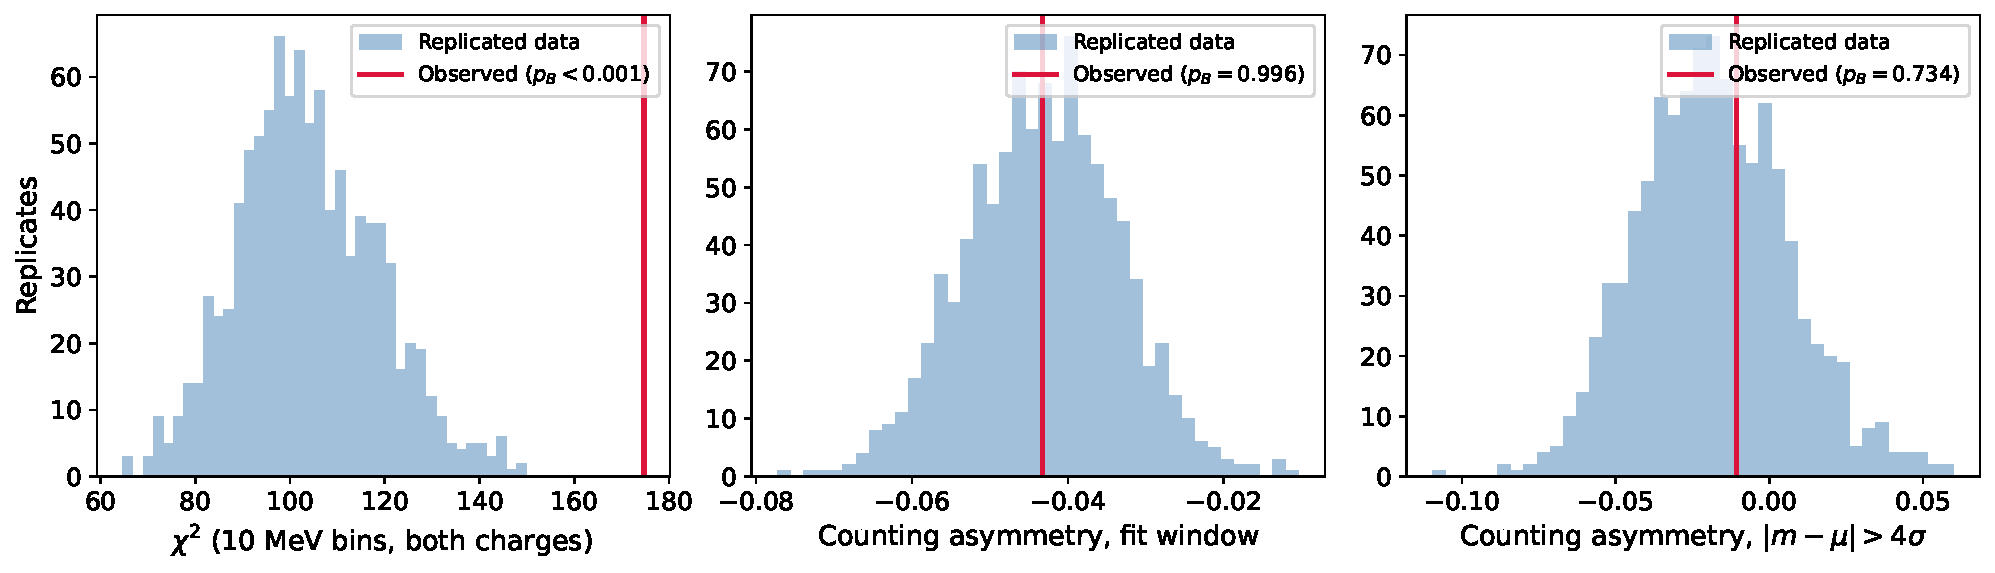
\includegraphics[width=0.95\textwidth]{figures/bayes_nominal_ppc.pdf}
\caption{Posterior predictive check: distributions of three discrepancies over $1000$ datasets replicated from posterior draws, compared with the observed values. (a) binned $\chi^2$; (b) and (c) counting asymmetry of the fit window and of the sidebands.}
\label{fig:bayes_ppc}
\end{figure*}

The binned $\chi^2$ uses the posterior medians only. A posterior predictive check~\cite{gelman_ppc} accounts for the posterior uncertainty and tests specific features of the data: for $1000$ parameter sets $\theta_j$ drawn from the posterior, a dataset $y^{\mathrm{rep}}_j$ is generated from the model, and a discrepancy $T(y,\theta_j)$ is computed both on the replica and on the data; the posterior predictive $p$-value is $p_B=P\big(T(y^{\mathrm{rep}},\theta)\geq T(y,\theta)\mid y\big)$. For the binned $\chi^2$ the replicas give $104\pm15$ and the data $175$ (median over $\theta_j$): none of the replicas reaches the observed value ($p_B<10^{-3}$), with the misfit concentrated in the $B^+$ sample ($p_B<10^{-3}$, against $0.03$ for $B^-$). The counting asymmetries of the whole window ($p_B=0.996$) and of the signal window ($0.99$) are reproduced, but this is expected and not informative: $A$ is a free parameter, so the replicas are centred on the observed value by construction. The asymmetry of the sidebands ($0.73$), which the fit constrains less directly, is also reproduced (Fig.~\ref{fig:bayes_ppc}). The check therefore shows that the model misdescribes the shape of the spectrum, mainly the signal tails, and does not reveal a charge-dependent distortion of the sidebands; that $\Araw$ does not depend on the signal shape is shown directly by its stability under the Crystal Ball model (Table~\ref{tab:gof}).

\subsection{Robustness Checks: Polarity, Prior and Charm Vetoes}
\label{sec:bayes_checks}
\emph{In short: $\Araw$ agrees between the two magnet polarities ($0.7\sigma$) and does not depend on the prior; the $D^0$ veto moves it by $2.3$ times the expected statistical spread.}
\begin{figure}[h]
\centering
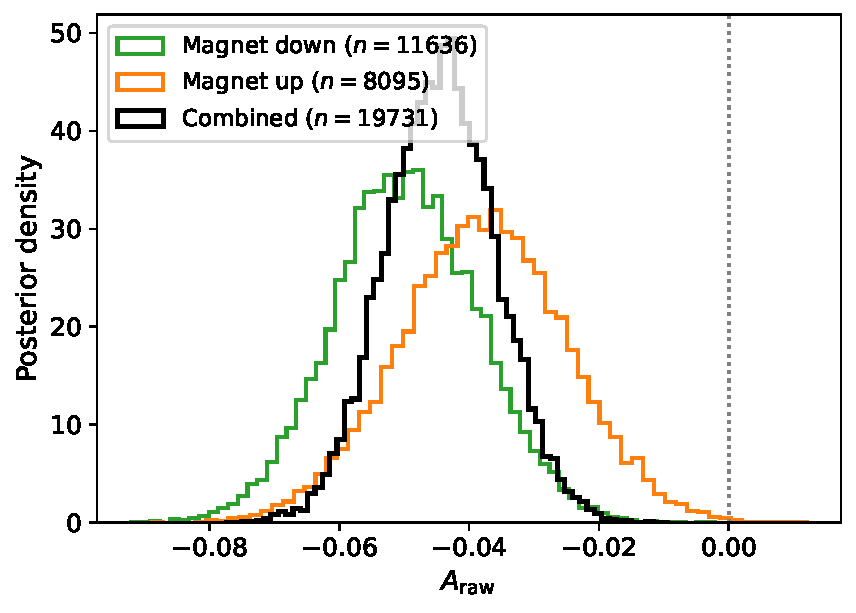
\includegraphics[width=\columnwidth]{figures/bayes_nominal_magnet.pdf}
\caption{Posterior of $\Araw$ for the magnet-down, magnet-up and combined samples.}
\label{fig:bayes_magnet}
\end{figure}

The fit was repeated separately on the two magnet polarities, whose left-right detection asymmetries are opposite and partially cancel in the combined sample: $\Araw(\text{down})=-0.0497\pm0.0112$ ($n=11{,}636$) and $\Araw(\text{up})=-0.0378\pm0.0129$ ($n=8095$); the frequentist fits give $-0.0492\pm0.0111$ and $-0.0374\pm0.0131$, and the sum of their profile likelihoods $-0.0443\pm0.0084$ (Appendix~\ref{sec:appendix_checks}). They differ by $0.7\sigma$, so there is no indication that the asymmetry is an artifact of one polarity (Fig.~\ref{fig:bayes_magnet}). A narrower prior, $A\in(-0.3,0.3)$, leaves the posterior unchanged ($\Araw=-0.0443$), as expected for a posterior far from the prior bounds; the prior width matters only for the Bayes factor (Sec.~\ref{sec:bayes_factor}).



The sample contains $B^\pm$ decays through intermediate charm states, $B^\pm\to D^0K^\pm$, $J/\psi K^\pm$ and $\chi_{c0}K^\pm$ with $D^0$, $J/\psi$, $\chi_{c0}\to K^+K^-$, which are visible as peaks in the opposite-sign $m(K^+K^-)$ spectra. They are part of the $B^\pm\to K^\pm K^+K^-$ final state and are kept in the nominal sample; removing them changes the observable, from the asymmetry of all $B^\pm\to K^\pm K^+K^-$ decays to that of the charmless ones, so the vetoes are reported as an informative check rather than as a systematic variation. A candidate is vetoed if either opposite-sign pair, $m(H1,H2)$ or $m(H1,H3)$, lies within $\pm30\,\MeV$ of the $D^0$ or $J/\psi$ mass or within $\pm60\,\MeV$ of the $\chi_{c0}$ mass (world-average masses; the wider window for the $\chi_{c0}$ reflects its natural width). The $D^0$ veto alone keeps $18{,}744$ candidates and gives $\Araw=-0.0496\pm0.0088$; the three vetoes together keep $16{,}367$ and give $-0.0423\pm0.0094$. The shifts with respect to the nominal fit, $-0.0053$ and $+0.0020$, compare with expected statistical fluctuations of $0.0023$ and $0.0040$ for a subsample of the nominal one (Sec.~\ref{sec:syst}); the $D^0$ veto moves $\Araw$ by $2.3$ times this amount, i.e.\ the vetoed $D^0K^\pm$ candidates have a less negative asymmetry than the rest of the sample. The analysis was also carried out with a minimal six-parameter model, with a narrower window and a single exponential background, before the nominal model was fixed; it gives a compatible result (Appendix~\ref{sec:bayes_minimal}).

\subsection{Toy-MC Coverage Validation}
\label{sec:bayes_toymc}
\emph{In short: $200$ toy-MC experiments give coverage $0.65\pm0.03$ ($68\%$) and $0.93\pm0.02$ ($95\%$), consistent with nominal, with unbiased estimates and pulls of width $1.04$.}
\begin{figure}[h]
\centering
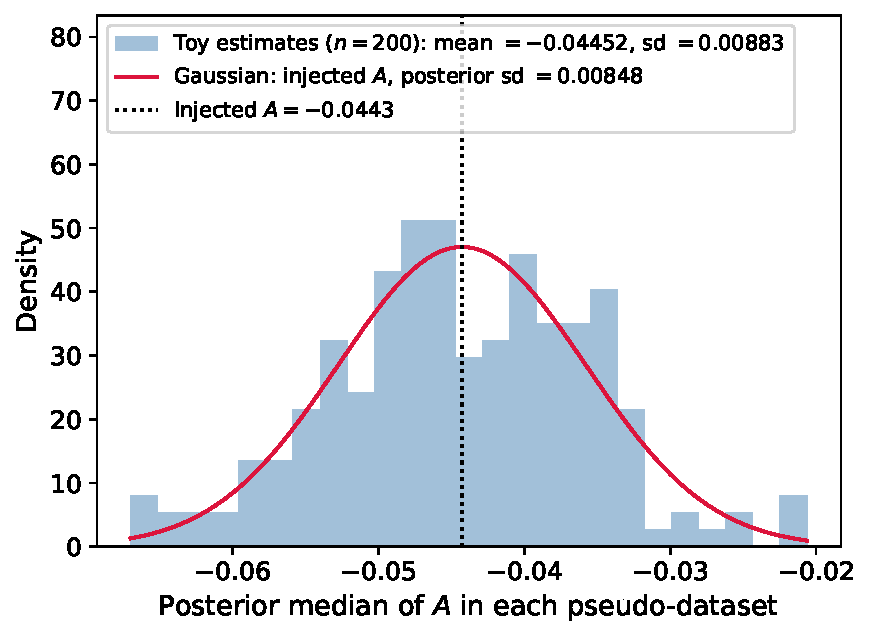
\includegraphics[width=\columnwidth]{figures/bayes_nominal_toys.pdf}
\caption{Toy-MC validation, 200 toy-MC datasets. (a) Pulls $(\hat A-A_{\mathrm{true}})/\sigma(\hat A)$, with $\hat A$ and $\sigma(\hat A)$ the posterior median and standard deviation of each replica, compared with a standard normal. (b) Fraction of replicas whose 68\% and 95\% credible intervals contain the injected value, with binomial uncertainties, and the nominal coverage.}
\label{fig:bayes_toys}
\end{figure}

The two kinds of interval have different meanings. A Bayesian credible interval is a statement about the parameter given the observed data and the prior: the true $A$ lies in it with the stated probability. A frequentist confidence interval, such as the profile-likelihood interval of Sec.~\ref{sec:frequentist}, is obtained by inverting a hypothesis test: the parameter is fixed and the interval is the random quantity, which changes from one repetition of the experiment to the next, and the confidence level is the fraction of repetitions in which it contains the true value (its coverage); it is not the probability that the true value lies in the interval observed. With flat priors and $\sim2\times10^4$ events the two intervals coincide numerically (Sec.~\ref{sec:bayes_posterior}), but only the confidence interval has the nominal coverage by construction, and only asymptotically; nothing guarantees it for the credible interval. To check this, 200 toy-MC datasets were generated from the fitted model (parametric bootstrap, with the posterior medians as ground truth and Poisson-fluctuated yields for each charge and component; the truncated Gaussian and exponential masses are drawn with the transformation method, i.e.\ by inverting their cumulative distributions) and each was refit with the nominal procedure and a $12{,}000$-step chain. The fraction of replicas whose interval contains the injected $A$ is $0.650\pm0.033$ for the 68\% CI and $0.930\pm0.015$ for the 95\% CI (binomial uncertainties), $1.0\sigma$ and $1.3\sigma$ below nominal: the coverage is consistent with nominal. The estimates themselves are unbiased and their spread matches the reported uncertainty (Fig.~\ref{fig:bayes_toys}): their mean differs from the injected value by $-0.0002\pm0.0006$, their standard deviation, $0.0088$, agrees with the posterior standard deviation of the data fit, $0.0085$, and the pulls have mean $-0.03\pm0.07$ and standard deviation $1.04$.

The toy chains are shorter than the nominal one, and in 124 of the 200 replicas the slowest-mixing parameter, always a background-shape parameter, has $N/\tau<50$ (median $48$, minimum $22$). The criterion on the slowest parameter is conservative for the quantity tested here: for $A$ itself the median autocorrelation time is $156$ steps, so each chain is at least $45$ autocorrelation times long in $A$ and provides $\gtrsim1400$ effectively independent samples of it. The Monte Carlo error on the percentiles of $A$ is then a few per cent of $\sigma(A)$, negligible against the binomial uncertainty of the coverage, and the replicas with $N/\tau<50$ do not show a lower coverage than the others ($0.69$ for the $68\%$ interval, against $0.58\pm0.06$ for the $76$ replicas with $N/\tau\geq50$, whose coverage is $1.9$ standard deviations below nominal: the split was made after the fact and $200$ replicas cannot tell a trend from a fluctuation, and the check on the data of Sec.~\ref{sec:freq_coverage} gives the nominal coverage). This is a closure test of the inference procedure: since the toys are generated from the same model that is fitted, it does not probe the model mismatch of Sec.~\ref{sec:bayes_gof}, which is instead addressed by the systematic study.

\FloatBarrier


\section{Stability Scans of the Frequentist Analysis}
\label{app:ext_syst}
\subsection{Stability Scans of the Frequentist Analysis}
\label{sec:syst_scans}
\emph{In short: the fit does not depend on the fit window or on the signal region, and the only dependence that matters is the one on the particle-identification requirements.}
The frequentist fit was also repeated on two-dimensional grids of the selection and fit settings (Sec.~\ref{sec:freq_syst}), with the nominal double-exponential model at each point. These scans test the stability of $\Araw$ and do not enter the systematic uncertainty, whose variants and combination rule are those above. Three results are used here, from the same notebook as the nominal fit.
\begin{itemize}[leftmargin=*,itemsep=1pt]
\item \emph{Fit window}: the maximum shift with respect to the nominal fit is $0.0048$ over the grid of lower and upper edges (standard deviation $0.0018$, mean statistical uncertainty $0.0085$); the extreme corners are the smallest and most asymmetric windows, where the background shape is least constrained.
\item \emph{Signal region} (used only to start the sideband fit): the shift is at most $6\times10^{-5}$, so the result does not depend on it.
\item \emph{Particle-identification requirements}: on the grid of the two cuts the maximum shift is $0.0126$ (standard deviation $0.0046$). This is larger than the statistical uncertainty of the nominal fit, $0.0085$, but the grid contains much smaller samples, with a mean statistical uncertainty of $0.0112$; the relevant comparison for nested samples is with $\sigma_B$, as in the one-cut-at-a-time scan above, where no shift exceeds $1.3\,\sigma_B$ on the tight side.
\end{itemize}
The window and signal-region scans are therefore consistent with a fit that does not depend on these choices, and the preselection remains the dominant contribution, as quantified by the systematic study.

\FloatBarrier


\section{Extended Validation of the Estimator}
\label{app:ext_valid}
\subsection{Size and Power of the Test of $A=0$}
\label{sec:validation_power}
\emph{In short: the test has the nominal size, the statistic $q(0)$ follows a $\chi^2$ distribution with one degree of freedom, and an asymmetry of $-0.02$ would be rejected at $3\sigma$ in one toy-MC experiment out of four.}
Under $A_{\mathrm{true}}=0$ the fraction of toy-MC experiments with $q(0)>3.84$ is $0.051\pm0.013$, against the nominal size $\alpha=0.05$, and $2$ of $293$ exceed $q=9$ ($3\sigma$), against the $0.8$ expected; the distribution of $q(0)$ is compatible with $\chi^2_1$ (Kolmogorov-Smirnov $p=0.79$, Fig.~\ref{fig:validation_null}a), and the tail used for the significance ($q=27$) is an extrapolation of it. The power, the probability of rejecting $A=0$ when the asymmetry is $A_{\mathrm{true}}$ (Fig.~\ref{fig:validation_injection}c), is $1.00$ at the fitted value and at $\pm$ the larger injected values, and $0.68$ ($0.27$ at $3\sigma$) at $A_{\mathrm{true}}=-0.02$: with $19{,}731$ candidates an asymmetry of $0.02$ is detected in about two experiments out of three at the $5\%$ size, and an asymmetry below that is not resolved.

\begin{figure*}[!t]
\centering
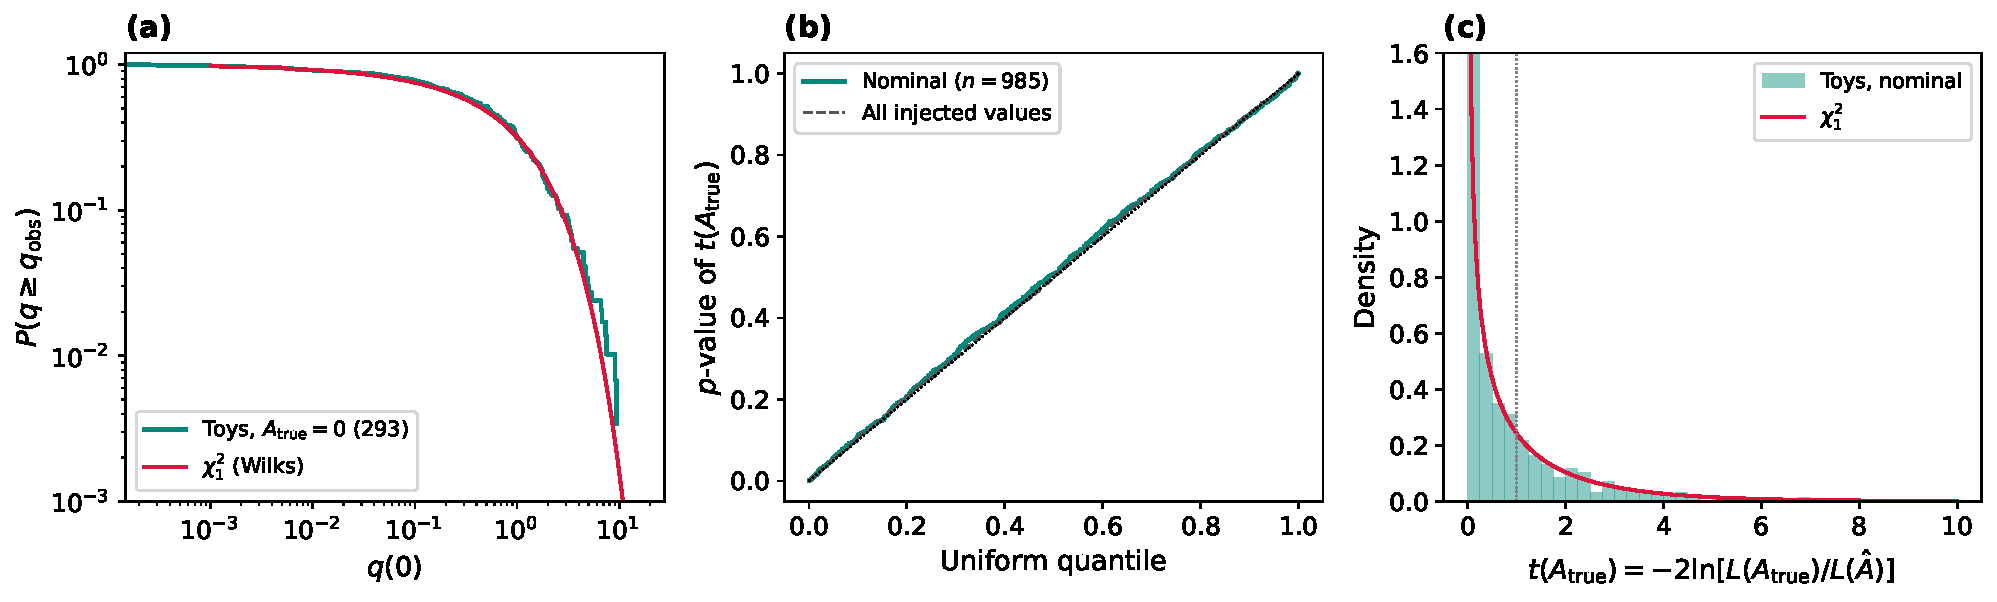
\includegraphics[width=0.95\textwidth]{figures/validation_null_wilks.pdf}
\caption{Toy-MC experiments, validity of Wilks' theorem. (a) Fraction of experiments with $q(0)$ above the observed value, for $A_{\mathrm{true}}=0$, compared with the $\chi^2_1$ distribution. (b) $p$-value of $t(A_{\mathrm{true}})$ against a uniform distribution, at the fitted value and pooled over the injected values. (c) Distribution of $t(A_{\mathrm{true}})$ at the fitted value and $\chi^2_1$.}
\label{fig:validation_null}
\end{figure*}



\begin{figure*}[!t]
\centering
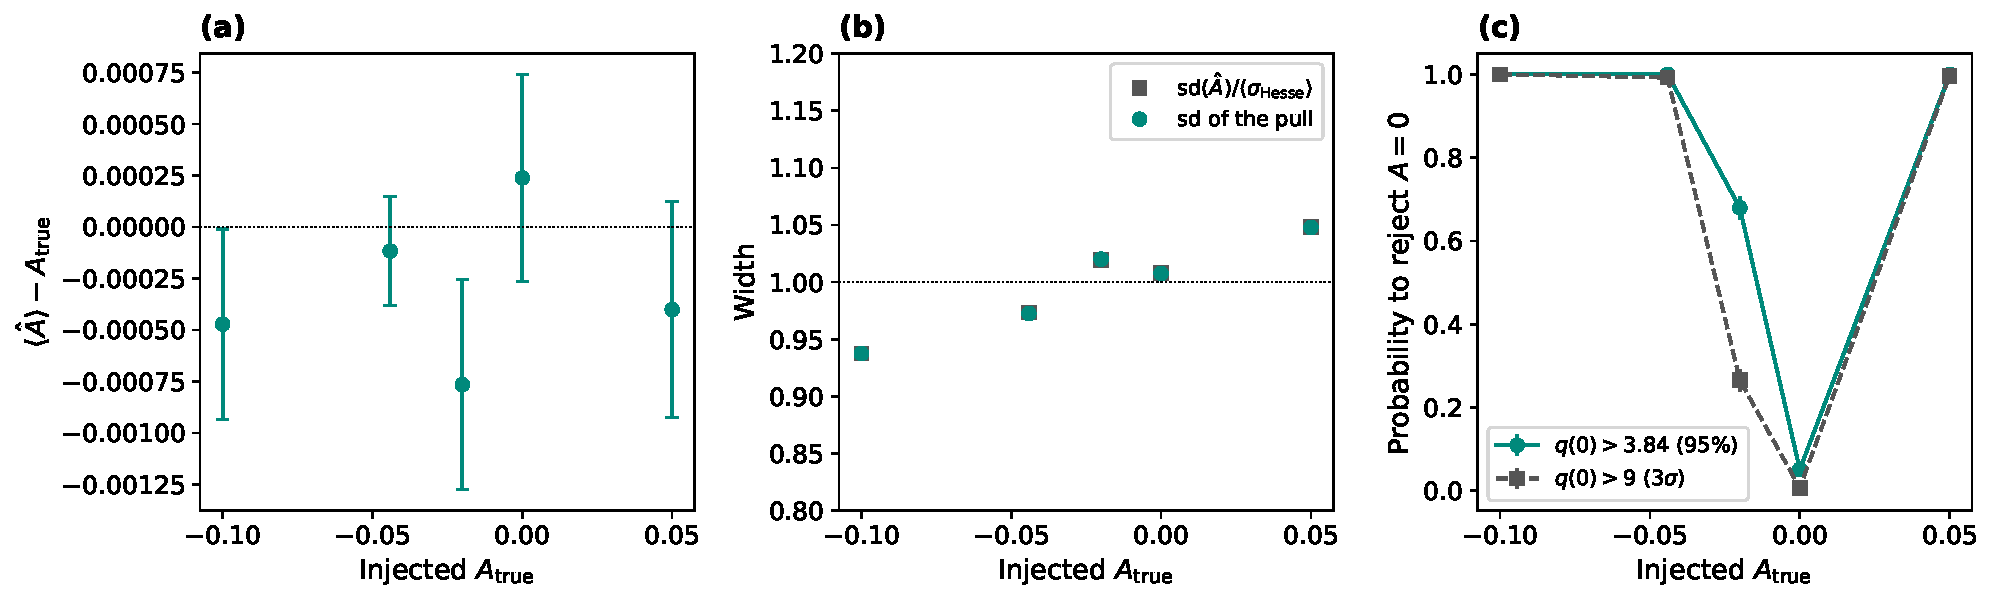
\includegraphics[width=0.95\textwidth]{figures/validation_injection_power.pdf}
\caption{Toy-MC experiments at five injected asymmetries. (a) Bias of $\hat A$, with its standard error. (b) Spread of the estimates divided by the mean Hesse uncertainty, and width of the pulls. (c) Probability to reject $A=0$ in the test with $q(0)>3.84$ (size $5\%$) and $q(0)>9$ ($3\sigma$), as a function of the injected value: size at $A_{\mathrm{true}}=0$, power elsewhere.}
\label{fig:validation_injection}
\end{figure*}

\subsection{Goodness of Fit and the Binning}
\label{sec:validation_gof}
\emph{In short: the binned $\chi^2$ of toy-MC experiments follows its asymptotic distribution, so its $p$-values are accurate; the misfit of the data is $5.4$ standard deviations at $10\,\MeV$ bins and $2.0$ at $2.5\,\MeV$, because it lives on the scale of the flanks of the peak.}
The $p$-values of the binned $\chi^2$ rely on the asymptotic distribution with $\mathrm{ndof}$ degrees of freedom, which can fail for bins with few entries. The $\chi^2$ of $1000$ toy-MC experiments from the fitted model has mean $87.6$ and standard deviation $13.3$ for $2\times50$ bins ($88$ degrees of freedom, expected $\sqrt{2\cdot88}=13.3$), and mean $387.6$, standard deviation $27.1$ for $2\times200$ bins ($388$ degrees of freedom): the asymptotic $\chi^2$ distribution describes the toys (Fig.~\ref{fig:validation_gof}). The data give $159.5$ for $2\times50$ bins of $10\,\MeV$, $5.4$ standard deviations above the toys (asymptotic $p=4.8\times10^{-6}$, fewer than $1/1000$ toys above), $253.1/188$ for $5\,\MeV$ bins ($p=1.1\times10^{-3}$) and $441.7/388$ for $2.5\,\MeV$ bins ($2.0$ standard deviations, $p=0.031$, in toys $0.032$). The same fit therefore has $p=0.03$ or $p=5\times10^{-6}$ depending on the binning: the discrepancy between model and data is a feature of $\sim10\,\MeV$ width, the flanks of the peak (Fig.~\ref{fig:bayes_fit}), diluted in narrower bins, and the binned $\chi^2$ is a test whose power depends on the binning, in the same way as the Bayes factor depends on the prior width.

\begin{figure*}[!t]
\centering
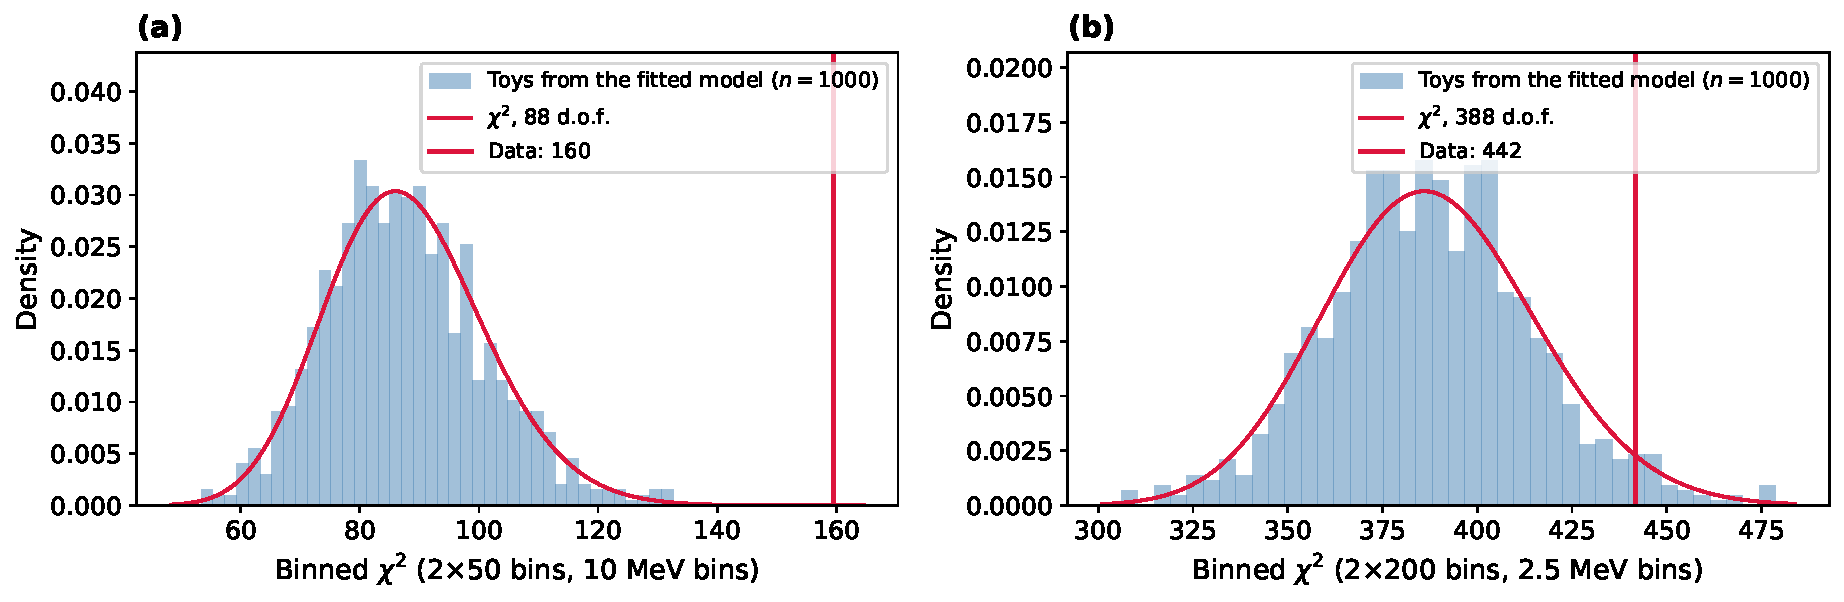
\includegraphics[width=0.95\textwidth]{figures/validation_gof_toys.pdf}
\caption{Binned $\chi^2$ of $1000$ toy-MC experiments from the fitted model, $\chi^2$ distribution with the corresponding degrees of freedom, and value of the data: (a) $2\times50$ bins of $10\,\MeV$, (b) $2\times200$ bins of $2.5\,\MeV$.}
\label{fig:validation_gof}
\end{figure*}

\FloatBarrier


\section{Extended Dalitz-Plane Analysis}
\label{app:ext_dalitz}
\subsection{Null Tests of the Local-Asymmetry Procedure}
\label{sec:dalitz_null}
Two null tests check the procedure itself. Shuffling the charges among the candidates removes any local asymmetry while keeping the occupancy of the bins and the global asymmetry of the data: over $2000$ permutations the $8\times8$ grid gives $\chi^2=31.4\pm8.1$, as expected for 31 degrees of freedom, and no permutation reaches the observed value (permutation $p<5\times10^{-4}$; $p=1\times10^{-3}$ for the $12\times12$ grid). The phase-space simulation of the record, without asymmetry by construction, gives $\chi^2=40.0/30$ ($p=0.11$) with the same procedure on the whole sample; on $500$ subsamples of the size of the data the mean $\chi^2/\mathrm{ndof}$ is $1.16$ and $13\%$ have $p<0.05$, so the $\chi^2$ $p$-values are slightly optimistic (the binomial uncertainty is evaluated at the observed $A_i$). The permutation test, whose null distribution is exact, gives the same conclusion: the non-uniformity is a property of the data.

\FloatBarrier


\section{Extended Machine Learning Module}
\label{app:ext_ml}
\subsection{Model Comparison}
\label{sec:ml_models}
\emph{In short: six classifiers; the tree ensembles and the neural network reach test AUC $0.857$--$0.864$, about $0.09$ above the linear models and indistinguishable from each other within the test-set uncertainty ($0.012$); gradient boosting, best in cross-validation, is the reference.}
\begin{table}[h]
\centering
\begin{tabular}{lccc}
\toprule
Model & CV AUC & Test AUC & Brier \\
\midrule
Logistic Regression       & $0.769 \pm 0.016$ & $0.771 \pm 0.013$ & $0.197$ \\
Logistic Regression (L1)  & --                & $0.771 \pm 0.013$ & $0.198$ \\
Decision Tree             & $0.816 \pm 0.011$ & $0.824 \pm 0.013$ & $0.133$ \\
Random Forest             & $0.863 \pm 0.017$ & $0.860 \pm 0.012$ & $0.122$ \\
Gradient Boosting         & $\mathbf{0.866 \pm 0.016}$ & $0.864 \pm 0.012$ & $0.116$ \\
FFNN                      & --                & $0.857 \pm 0.012$ & $0.134$ \\
\bottomrule
\end{tabular}
\caption{Cross-validated AUC (mean and standard deviation over the folds), test-set AUC (with bootstrap uncertainty) and test-set Brier score of the raw scores. Gradient boosting, best in cross-validation, is the reference model. The FFNN is validated on the validation set instead of by cross-validation.}
\label{tab:ml_models}
\end{table}

Six classifiers were trained: logistic regression, without and with an $L1$ penalty (linear baselines), a decision tree (depth 4, fixed in advance as a shallow, interpretable baseline and not pruned), a Random Forest~\cite{breiman_rf} (300 trees of depth 8), gradient boosting~\cite{friedman_gbm} (200 stages of depth-3 trees, learning rate $0.05$), and a feed-forward neural network (FFNN: two hidden layers of 32 and 16 units with ReLU activation, dropout $0.2$, binary cross-entropy, the Adam optimizer~\cite{adam} with learning rate $10^{-3}$, early stopping on the validation AUC, sigmoid output). The linear models and the network are parametric, with a fixed number of parameters, and the trees and ensembles non-parametric, whose complexity grows with the data; the more flexible models are less interpretable, which is why the linear and single-tree baselines are kept. Both the logistic-regression log-loss and the network's binary cross-entropy are the negative log-likelihood of a Bernoulli distribution with probability $p(x)$, the same quantity minimized by the mass fits. The models are compared through the area under the receiver operating characteristic (ROC) curve (AUC), which equals the probability that a randomly chosen signal-like candidate receives a higher score than a randomly chosen background-like one ($0.5$ for a random classifier, $1$ for a perfect one). Table~\ref{tab:ml_models} gives the 5-fold cross-validated AUC on the training set and the AUC on the untouched test set, with its bootstrap uncertainty. The reference model for the rest of the section was chosen on the cross-validated AUC, so that the test set is not used for any choice: gradient boosting ($0.866$), essentially tied with the Random Forest ($0.863$).



\begin{figure}[h]
\centering
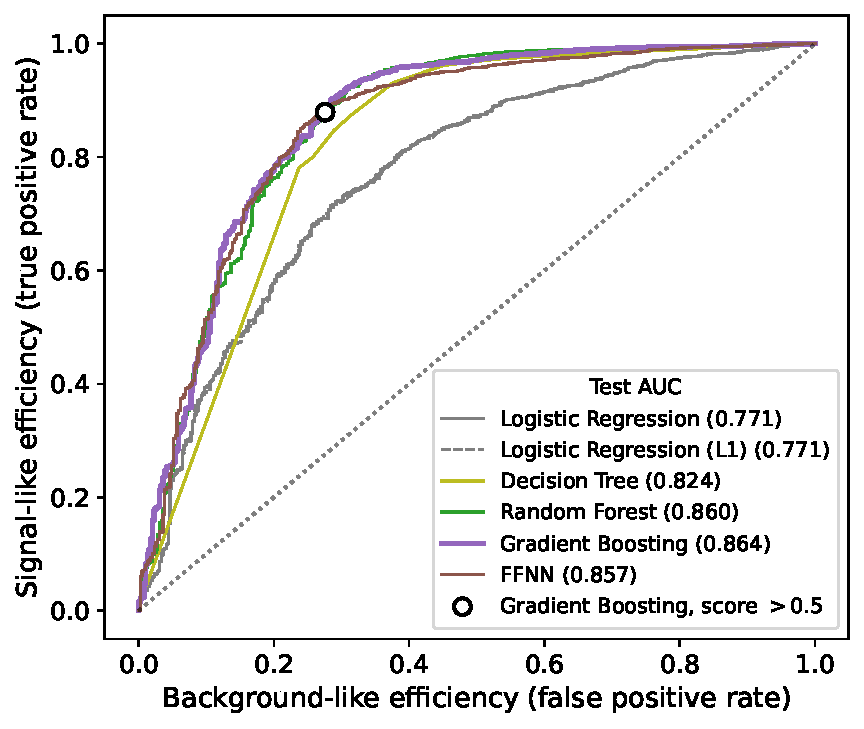
\includegraphics[width=\columnwidth]{figures/ml_nominal_roc.pdf}
\caption{ROC curves on the test set, with the test AUC of each model in the legend (Table~\ref{tab:ml_models}); the reference model is drawn thicker, and the two logistic regressions overlap. The circle marks the cut on the reference score used in Sec.~\ref{sec:ml_stability}.}
\label{fig:ml_roc}
\end{figure}

The three non-linear ensembles and the FFNN improve the AUC by $\sim$0.09 over the linear models and by $\sim$0.04 over the single tree (Fig.~\ref{fig:ml_roc}), while their mutual differences ($\leq0.007$) are smaller than the test-set uncertainty ($0.012$). The FFNN training is reproducible (fixed seeds, deterministic operations); its dependence on the random initialization, measured by retraining it with ten seeds, is $0.854\pm0.005$ in test AUC.



\begin{figure*}[t]
\centering
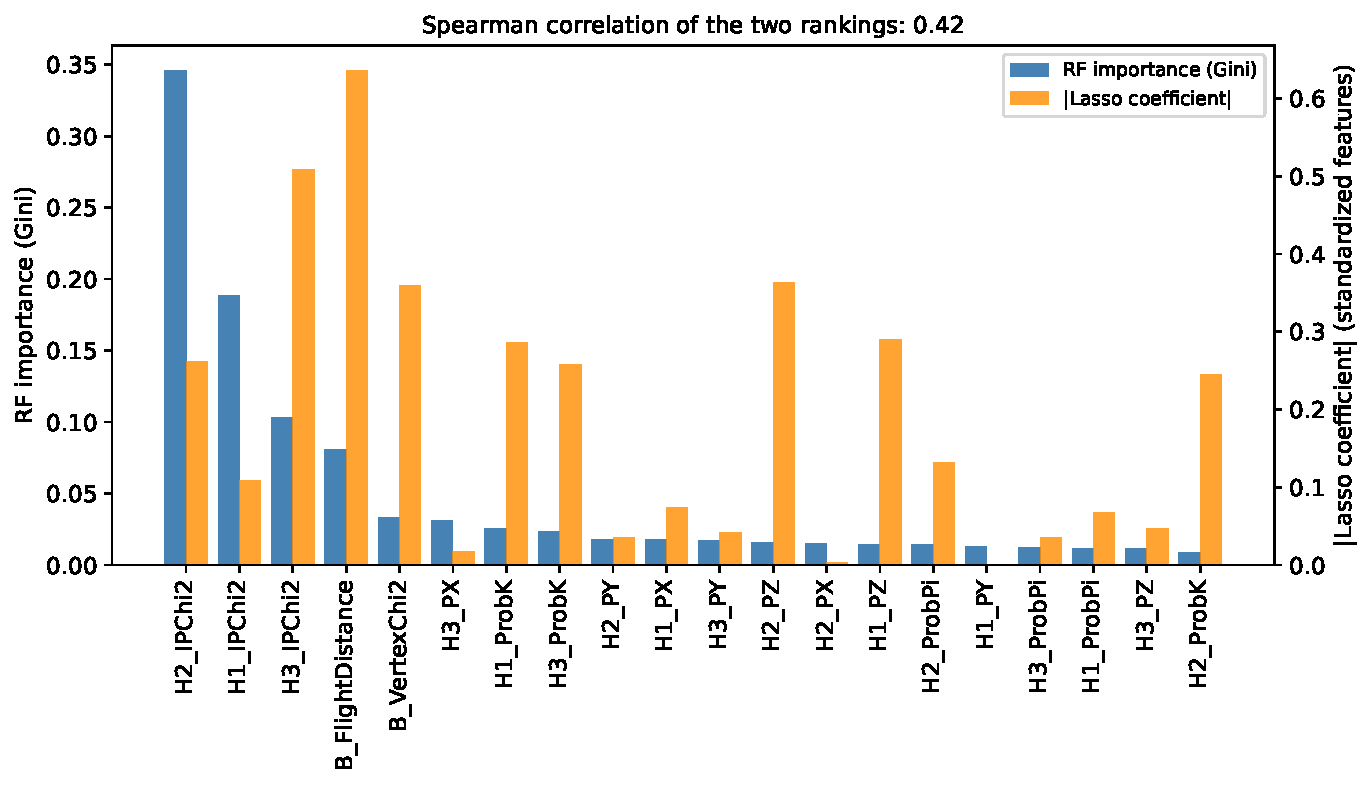
\includegraphics[width=0.95\textwidth]{figures/ml_nominal_features.pdf}
\caption{Random Forest feature importance (Gini, a) and magnitude of the Lasso coefficient of the standardized feature (b) for the 20 features, both ordered by Random Forest importance; the two $B$-candidate variables are highlighted.}
\label{fig:ml_features}
\end{figure*}

The two measures of the relevance of a feature available here -- the Random Forest importance (the decrease in Gini impurity $G=1-\sum_c p_c^2$, $p_c$ the class fractions in a node, produced by the splits on that feature) and the magnitude of the $L1$-regularized (Lasso~\cite{tibshirani_lasso}) logistic-regression coefficient of the standardized feature -- agree only partly (Fig.~\ref{fig:ml_features}; Spearman correlation of the two rankings $0.42$, $p=0.06$). The impact-parameter variables \texttt{IPChi2} dominate the Random Forest, while the Lasso coefficients are largest for \texttt{B\_FlightDistance}, \texttt{H3\_IPChi2}, \texttt{H2\_PZ} and \texttt{B\_VertexChi2}. The difference is expected: the Gini importance reflects the use of a feature in non-linear splits and interactions, and is shared among correlated features, while a linear coefficient measures the effect of a feature with the others held fixed. Both measures rank the two $B$-candidate variables among the top five (Random Forest 4th and 5th, Lasso 1st and 4th): they summarize in one number the displaced-vertex topology that the per-track variables encode only jointly.

\subsection{Regularization, Bias-Variance, and Calibration}
\label{sec:ml_regcal}
\emph{In short: the linear model does not overfit, gradient boosting overfits beyond $\sim$150 stages without losing test AUC, and class weights bias the probabilities, which an isotonic recalibration corrects (Brier score $0.122\to0.062$) without changing the ranking.}
A scan of the regularization strength of the logistic regression ($30$ log-spaced values of $C=1/\alpha$, cross-validated) gives the same optimal AUC for the $L1$ and $L2$ penalties ($0.7686$, at $C_{L1}=0.12$ and $C_{L2}=9.2$), and the optimal $L1$ penalty sets no coefficient to zero: the linear model does not overfit, and its limitation is the linear decision boundary, not the variance.

\begin{figure*}[t]
\centering
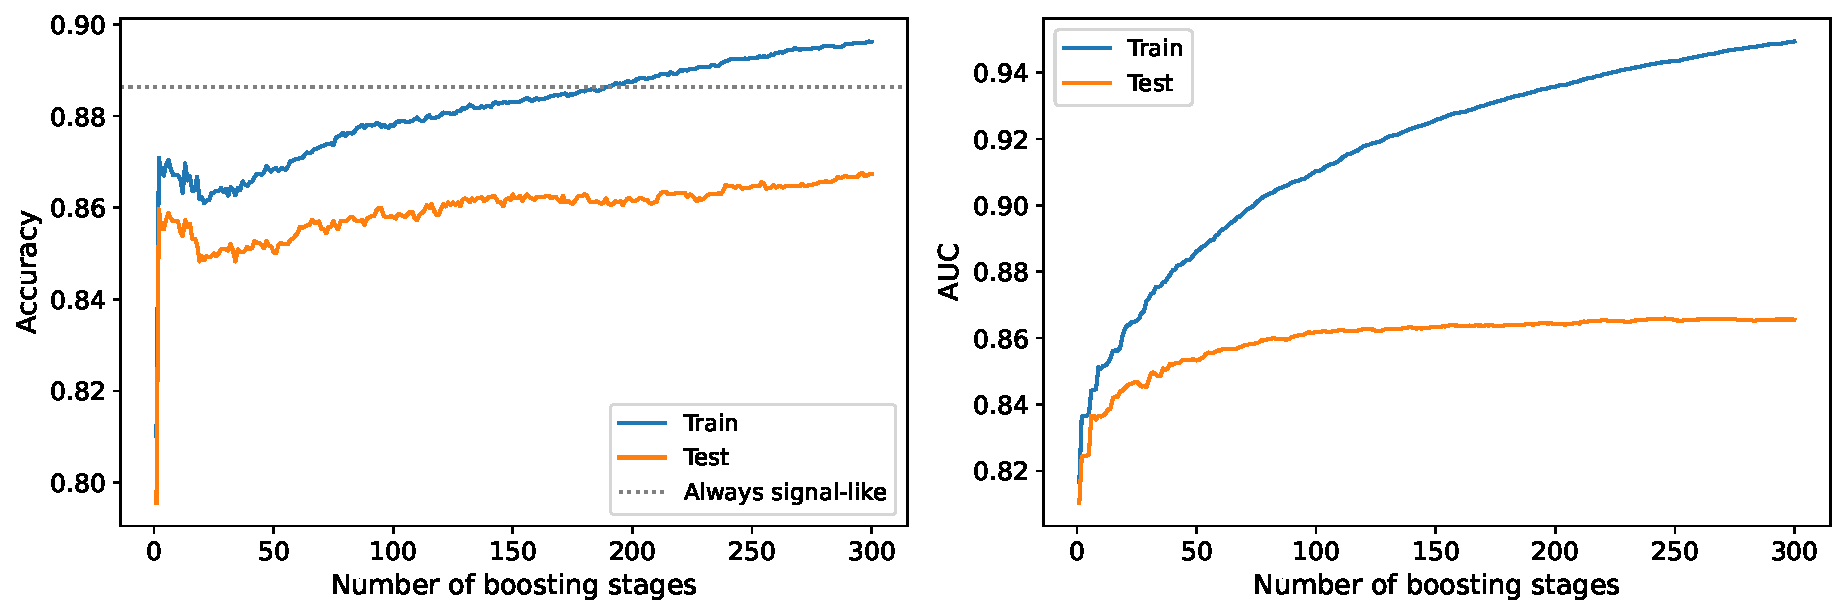
\includegraphics[width=0.95\textwidth]{figures/ml_nominal_bias_variance.pdf}
\caption{Gradient boosting: (a) accuracy at the $0.5$ threshold and (b) AUC on the training and test sets as a function of the number of boosting stages. The dotted line is the accuracy of always predicting the signal-like class.}
\label{fig:ml_bias_variance}
\end{figure*}

\begin{figure}[t]
\centering
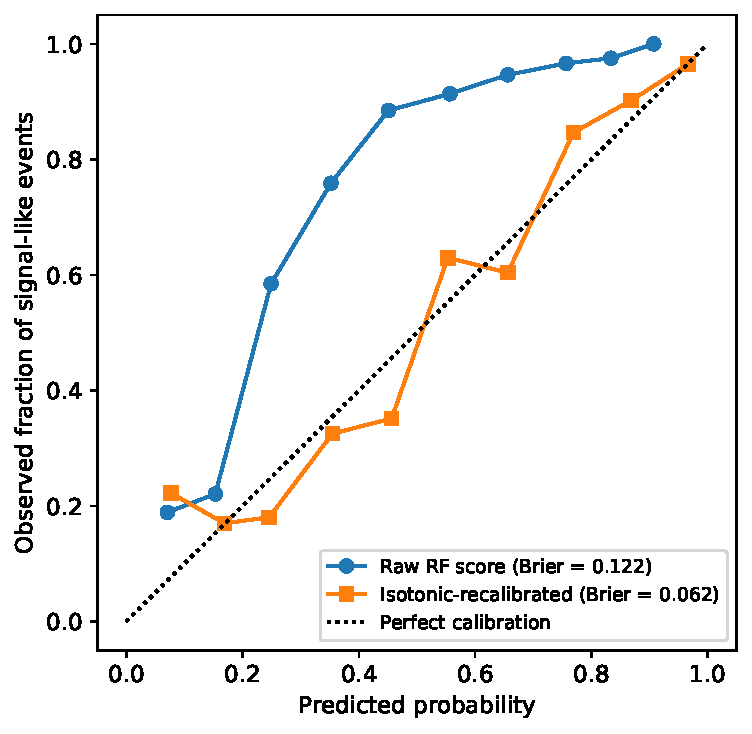
\includegraphics[width=\columnwidth]{figures/ml_nominal_calibration.pdf}
\caption{Reliability diagram of the Random Forest on the test set: observed fraction of signal-like candidates vs.\ predicted probability, for the raw score (with binomial uncertainties) and for the isotonic-recalibrated one. Bottom: distribution of the raw score for the two weak-label classes; the low-probability bins contain few candidates.}
\label{fig:ml_calibration}
\end{figure}

The bias-variance trade-off was studied with gradient boosting, whose complexity grows with the number of boosting stages (Fig.~\ref{fig:ml_bias_variance}). The test AUC rises up to $\sim$150 stages and then stays at $0.865$, while the training AUC keeps rising: the train-test gap grows from $0.018$ at 20 stages to $0.084$ at 300. The additional stages fit fluctuations of the training sample without improving the ranking of new candidates -- overfitting, which the default 200 stages of Table~\ref{tab:ml_models} do not reach in the test AUC. The test accuracy at the $0.5$ threshold stays below that of always predicting the majority class ($0.886$): with balanced class weights the classifier is trained to minimize the weighted error, in which a misclassified background-like candidate counts eight times more than a signal-like one, and not the unweighted error rate.




The AUC depends only on the ranking of the scores; whether a score can be read as a probability is measured by the Brier score~\cite{brier}, $\mathrm{BS}=\frac{1}{N}\sum_i (p_i-y_i)^2$, the mean squared difference between predicted probability $p_i$ and label $y_i\in\{0,1\}$ (lower is better). Class weights change the probabilities a model learns: a classifier trained with weights $w_s,w_b$ on the two classes converges to
\[
\tilde p=\frac{w_s p}{w_s p+w_b(1-p)}
\]
instead of the true $p$, i.e.\ it describes a world in which the classes are re-balanced. With $w_b>w_s$ the raw scores therefore \emph{underestimate} the probability of the signal-like class, which is what the reliability diagram of the Random Forest shows (Fig.~\ref{fig:ml_calibration}): at a raw score of $0.25$ the observed signal-like fraction is already $0.58$. An isotonic recalibration~\cite{zadrozny_elkan}, fitted on held-out folds of the unweighted training sample, follows the diagonal and halves the Brier score, from $0.122$ to $0.062$ (the Brier score is the mean squared error of the predicted probability against the $0/1$ label). Most of the gain undoes the re-weighting rather than correcting the model; the ranking, and hence the AUC and any selection based on a score threshold, is unchanged by a monotonic recalibration.

\subsection{Uncertainty Quantification}
\label{sec:ml_uncertainty}
\emph{In short: the three estimators give mean per-candidate uncertainties of $0.178$ (Random Forest), $0.095$ (MC dropout) and $0.050$ (deep ensemble); they measure different sources of variability, and only the Random Forest spread visibly decreases with the training-set size.}
\begin{figure*}[t]
\centering
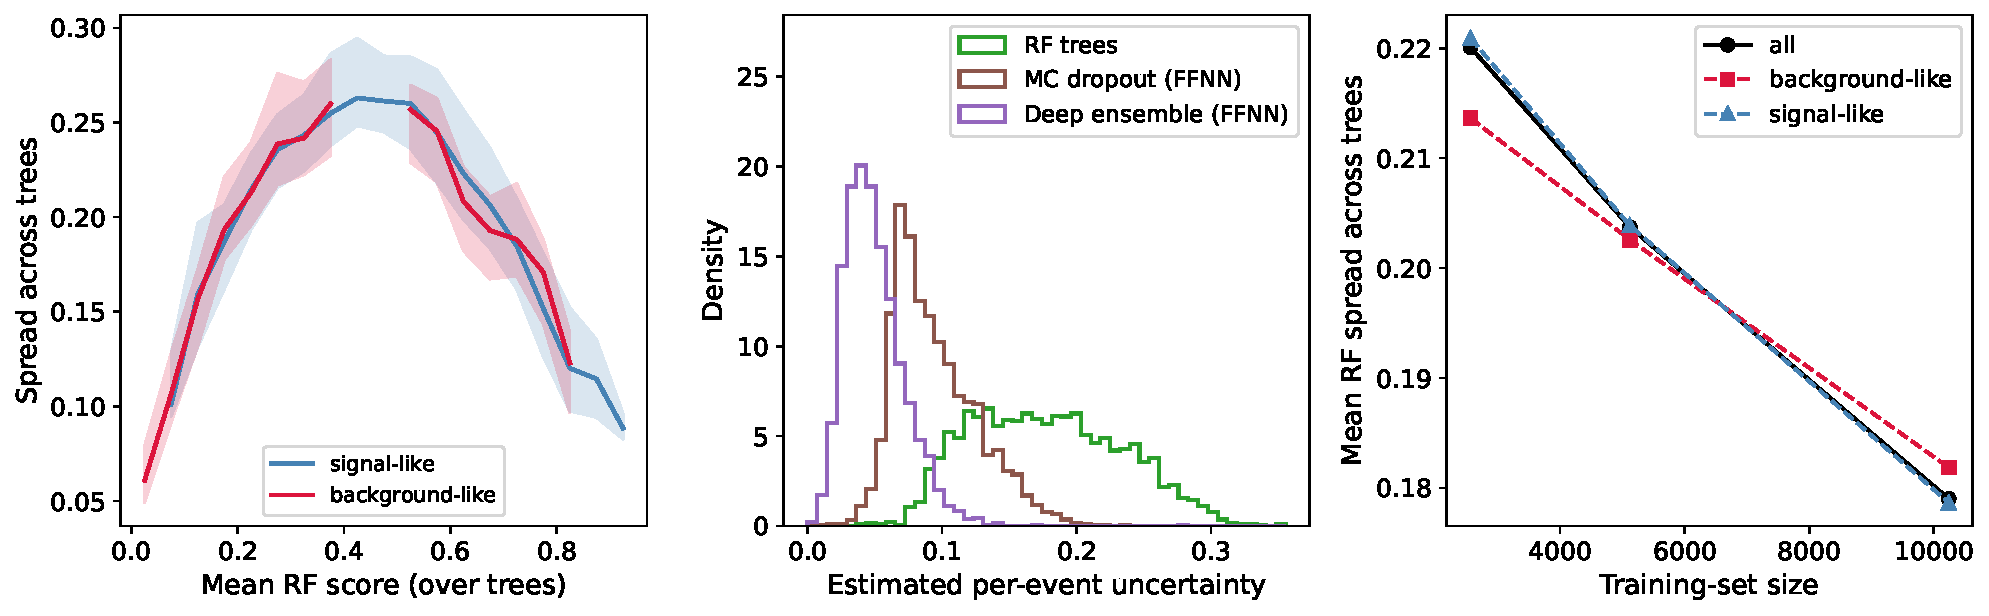
\includegraphics[width=0.95\textwidth]{figures/ml_nominal_uncertainty.pdf}
\caption{(a) Spread across the Random Forest trees vs.\ mean tree score, median and 16--84\% band of the test candidates of each weak-label class. (b) Distributions of the per-candidate uncertainty from the Random Forest trees, MC dropout and the deep ensemble. (c) Mean Random Forest spread vs.\ training-set size, for all, background-like and signal-like test candidates.}
\label{fig:ml_uncertainty}
\end{figure*}

The uncertainty of a prediction has two components: \emph{aleatoric}, from the intrinsic overlap of the classes in feature space, which more training data cannot reduce, and \emph{epistemic}, from the limited knowledge of the model parameters, which more training data reduces. Three estimators were compared, each giving an ensemble of $M$ predictions $p_m(x)$ for each candidate and quoting their spread, $\sigma(x)=\big[\frac1M\sum_m (p_m(x)-\bar p(x))^2\big]^{1/2}$: the $M=300$ trees of the Random Forest, each trained on a bootstrap sample; $M=300$ forward passes of the FFNN with dropout kept active at inference (MC dropout), which approximates sampling from a Bayesian posterior over the network weights~\cite{gal_mcdropout} (a full Bayesian network trained by variational inference was not used: it needs a dedicated implementation and MC dropout gives the same kind of ensemble at no extra cost); and a deep ensemble~\cite{deep_ensembles} of $M=10$ FFNNs trained from different random initializations. The mean per-candidate uncertainty is $0.178$ for the Random Forest, $0.095$ for MC dropout ($0.099\pm0.006$ over the ten initializations) and $0.050$ for the deep ensemble (Fig.~\ref{fig:ml_uncertainty}), with the same values within $10\%$ for background-like and signal-like candidates.

The three estimators answer different questions, which explains the factor $\sim$3.5 between them. The deep ensemble only varies the initialization, on the same training data; MC dropout also perturbs the network structure; the trees of the Random Forest differ in their training data (bootstrap) and in the features they use, and each tree, of limited depth, is individually a poor and discrete estimator of $p$. Their per-candidate values are correlated but not interchangeable (Spearman correlations $0.41$--$0.57$ between pairs). The Random Forest spread contains both components. It is largest for scores around $0.5$ (Fig.~\ref{fig:ml_uncertainty}a), where the classes overlap and the trees disagree most -- an aleatoric contribution; and it decreases with the size of the training set, from $0.220$ with a quarter of it to $0.204$ with half and $0.179$ with the full set, while the test AUC stays at $0.860$--$0.862$ -- the epistemic contribution, which more data reduces.

\subsection{K-means on the Dalitz Plot}
\label{sec:ml_kmeans}
\emph{In short: for $K=8$ two clusters deviate by more than $3\sigma$ ($\chi^2=46.4$ for $7$ degrees of freedom): a negative asymmetry at low $m^2_{\mathrm{lo}}$ and positive ones at high $m^2_{\mathrm{hi}}$, as in the fixed binning.}
$K$-means is the unsupervised part of the module: it uses no labels, and the partition of the Dalitz plane is learned from the density of the candidates rather than fixed by hand. As an adaptive alternative to the fixed Dalitz-plot binning of Sec.~\ref{sec:bayes_dalitz}, the candidates of the fit window were partitioned with $K$-means~\cite{lloyd_kmeans} on the two standardized Dalitz variables $(m^2_{\mathrm{lo}},m^2_{\mathrm{hi}})$. $K$-means partitions the points $x_i$ into $K$ clusters $C_k$ minimizing the within-cluster sum of squares (inertia) $W=\sum_k\sum_{i\in C_k}\lVert x_i-\bar x_k\rVert^2$, with $\bar x_k$ the cluster centroids; $K$ has to be fixed in advance. The quality of a partition is measured by the silhouette~\cite{silhouette}: for each point, $s_i=(b_i-a_i)/\max(a_i,b_i)$ compares its mean distance $a_i$ to the other points of its cluster with the mean distance $b_i$ to the points of the nearest other cluster, and the average over all points ($-1\le s\le 1$, higher is better) measures how well separated the clusters are. $K=8$ was fixed in advance, as a compromise between resolution and the number of candidates per cluster (at least $1233$), and $K=3$, the silhouette optimum over $K=2$--$12$ ($0.46$, against $0.41$ for $K=8$, a local maximum), was added. Both partitions are stable: repeating the clustering with a different random initialization gives an adjusted Rand index~\cite{hubert_ari} above $0.998$.

\begin{figure}[h]
\centering
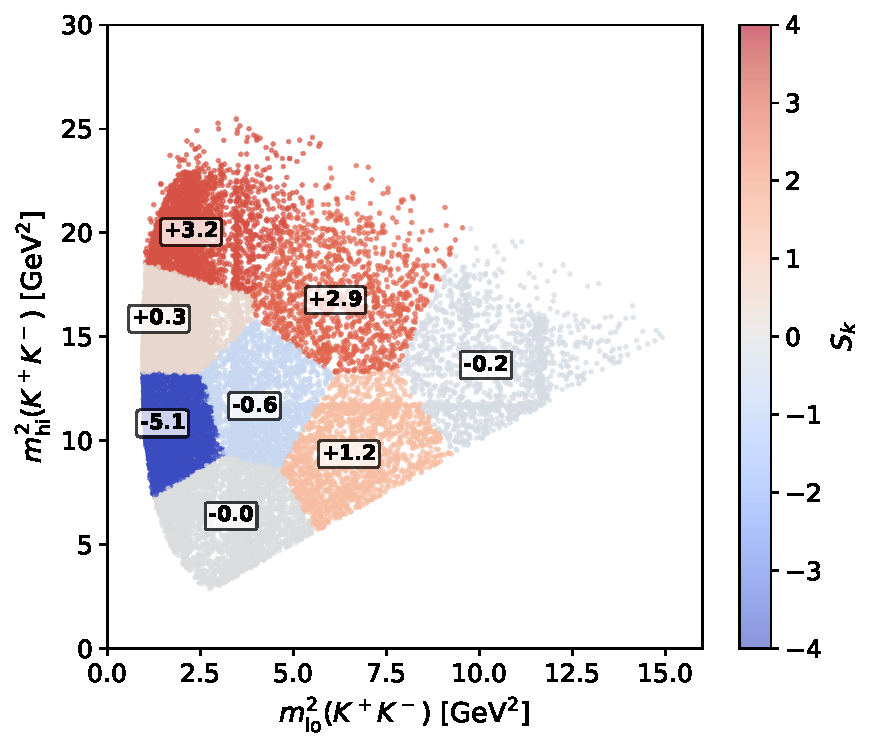
\includegraphics[width=\columnwidth]{figures/ml_nominal_kmeans.pdf}
\caption{$K$-means partition ($K=8$) of the Dalitz plane, all candidates of the fit window, same axes as Fig.~\ref{fig:bayes_dalitz}. Color and labels: local significance of each cluster with respect to the global asymmetry, $S_k=(A_k-A_{\mathrm{glob}})/\sigma(A_k)$, on the same scale as panel (c) of Fig.~\ref{fig:bayes_dalitz}.}
\label{fig:ml_kmeans}
\end{figure}

The asymmetry of each cluster was compared with the global one as in Sec.~\ref{sec:bayes_dalitz}, $S_k=(A_k-A_{\mathrm{glob}})/\sigma(A_k)$. For $K=8$ (Fig.~\ref{fig:ml_kmeans}), two clusters deviate by more than $3\sigma$ (probability $2\times10^{-4}$ for two or more if the asymmetry were uniform), and the homogeneity test gives $\chi^2=46.4/7$ ($p=7\times10^{-8}$). The most significant one lies at low $m^2_{\mathrm{lo}}$ ($1$--$2.5\,\GeV^2$) and intermediate $m^2_{\mathrm{hi}}$, with $A_k=-0.127\pm0.017$ ($n=3601$, $S_k=-5.1$); two clusters at high $m^2_{\mathrm{hi}}$ have positive asymmetries, $A_k=+0.020\pm0.020$ ($S_k=+3.2$) and $+0.040\pm0.028$ ($+2.9$). In the signal window ($|m-\mu|<2\sigma$) the same pattern is sharper -- three clusters beyond $3\sigma$, with $S_k=-5.6$, $+4.4$ and $+3.0$, and $\chi^2=62.3/7$ -- so it is not produced by the background. The coarser $K=3$ partition gives $\chi^2=15.2/2$ ($p=5\times10^{-4}$). The adaptive partition therefore confirms the picture of the fixed binning, a negative local asymmetry at low $m^2_{\mathrm{lo}}$ and positive ones at high $m^2_{\mathrm{hi}}$, with the same caveats (no background subtraction, no correction for detection asymmetries).

\subsection{Hyperparameter Optimization}
\label{sec:ml_hyper}
\emph{In short: the best configurations improve the test AUC by at most $0.005$, less than its uncertainty, and the cross-validated maximum overestimates the test AUC (winner's curse).}
The hyperparameters of the Random Forest ($120$ configurations), gradient boosting ($100$) and the FFNN ($168$: seven architectures, four dropout rates, six learning rates) were optimized by repeated cross-validation on the training set (Tables~\ref{tab:ml_hyperparams}--\ref{tab:ml_ffnn_search}). The best configurations improve the test AUC over the defaults of Table~\ref{tab:ml_models} by $0.005$ (Random Forest), $0.001$ (gradient boosting) and $0.004$ (FFNN), all well below the test-set uncertainty ($0.012$) and, for the FFNN, comparable with its spread over initializations ($0.005$). For the two tree ensembles the best cross-validated AUC is higher than the test AUC of the same configuration ($0.871$ vs $0.866$ and $0.868$ vs $0.865$), as expected when the maximum is taken over many noisy cross-validation estimates (the ``winner's curse''): the selection favors configurations with a favorable fluctuation, and the cross-validated score of the selected configuration is an optimistic estimate of its performance. The searches show that the defaults are already close to optimal for this problem, so the defaults are used throughout.

\begin{table*}[t]
\centering
\begin{tabular}{lp{7cm}lc}
\toprule
Model & Grid & Best configuration & CV AUC / Test AUC (default) \\
\midrule
Random Forest & \texttt{n\_estimators} $200$--$1200$, \texttt{max\_depth} $6$--$12$ or none, \texttt{min\_samples\_leaf} $5$--$40$ & $400$, $12$, $5$ & $0.8706$ / $0.8656$ ($0.8604$) \\
Gradient Boosting & \texttt{n\_estimators} $100$--$500$, \texttt{max\_depth} $1$--$5$, \texttt{learning\_rate} $0.01$--$0.1$ & $300$, $2$, $0.1$ & $0.8684$ / $0.8650$ ($0.8643$) \\
\bottomrule
\end{tabular}
\caption{Hyperparameter search for the tree ensembles ($120$ and $100$ configurations, 5-fold cross-validation repeated 10 times, balanced class weights). The test AUC of the best configuration is compared with that of the default of Table~\ref{tab:ml_models} (in parentheses); the bootstrap uncertainty of each test AUC is $0.012$.}
\label{tab:ml_hyperparams}
\end{table*}

\begin{table*}[t]
\centering
\begin{tabular}{llccc}
\toprule
Architecture & Layers & Dropout & Learning rate & CV AUC \\
\midrule
\texttt{deep\_3layer} (best) & $[64,32,16]$ & $0.2$ & $0.003$ & $0.8585\pm0.0174$ \\
\texttt{wide\_2layer}        & $[64,32]$    & $0.3$ & $0.003$ & $0.8582\pm0.0175$ \\
\texttt{deep\_3layer}        & $[64,32,16]$ & $0.3$ & $0.003$ & $0.8580\pm0.0187$ \\
\texttt{wide\_2layer}        & $[64,32]$    & $0.3$ & $0.005$ & $0.8579\pm0.0184$ \\
\texttt{wide\_2layer}        & $[64,32]$    & $0.4$ & $0.005$ & $0.8579\pm0.0187$ \\
\bottomrule
\end{tabular}
\caption{Top five of the $168$ FFNN configurations ($7$ architectures from one hidden layer of 8 units to five layers $[128,64,32,16,8]$, dropout $0.1$--$0.4$, learning rates $0.0002$--$0.005$; 5-fold cross-validation repeated twice). The five are within $0.0007$ of each other, far below the fold-to-fold spread: the optimum is a plateau. The best configuration has test AUC $0.8606$, against $0.8568$ for the default architecture ($\pm0.005$ over initializations).}
\label{tab:ml_ffnn_search}
\end{table*}

\subsection{High-Background Sample}
\label{sec:ml_highbkg}
In the nominal sample the selection cannot improve the precision because there is little background to remove. To test it where the background is larger, the same study was repeated on a sample with a looser kaon identification, $\texttt{ProbK}>0.3$ ($33{,}328$ candidates, signal purity $94\%$ within $\pm2\sigma$ of the peak), with the reference classifier retrained on the weak labels of this sample (test AUC $0.895$). Cleaning it with a cut on the classifier score is compared with tightening the identification cut, at equal signal efficiency (Fig.~\ref{fig:ml_high_bkg}). The classifier removes the combinatorial background with little signal loss -- a cut at $0.5$ keeps $93\%$ of the signal and raises the purity to $99\%$ -- and at any efficiency gives a slightly smaller $\sigma(\Araw)$ than the identification cut. The gain is small ($0.0072\to0.0070$ at best): loosening the identification adds mostly signal ($+47\%$ with respect to the nominal selection), and the background under the peak stays a small fraction. The classifier also cannot remove the background that matters for $\Araw$. With the looser identification the asymmetry moves to $-0.055$, as expected from misidentified $B^\pm\to\pi^\pm K^+K^-$ decays (Sec.~\ref{sec:syst}); tightening the identification cut to $\texttt{ProbK}>0.4$ moves it back by $+0.008$ ($3.3$ times the nested-sample spread), while the score cut that keeps $93\%$ of the signal moves it by $-0.001$. Misidentified $B$ decays peak close to the $B$ mass, so the mass-based weak labels mark them as signal-like: the CWoLa classifier, by construction, cannot learn to reject a background that sits under the peak, and particle identification remains necessary.


\begin{figure*}[t]
\centering
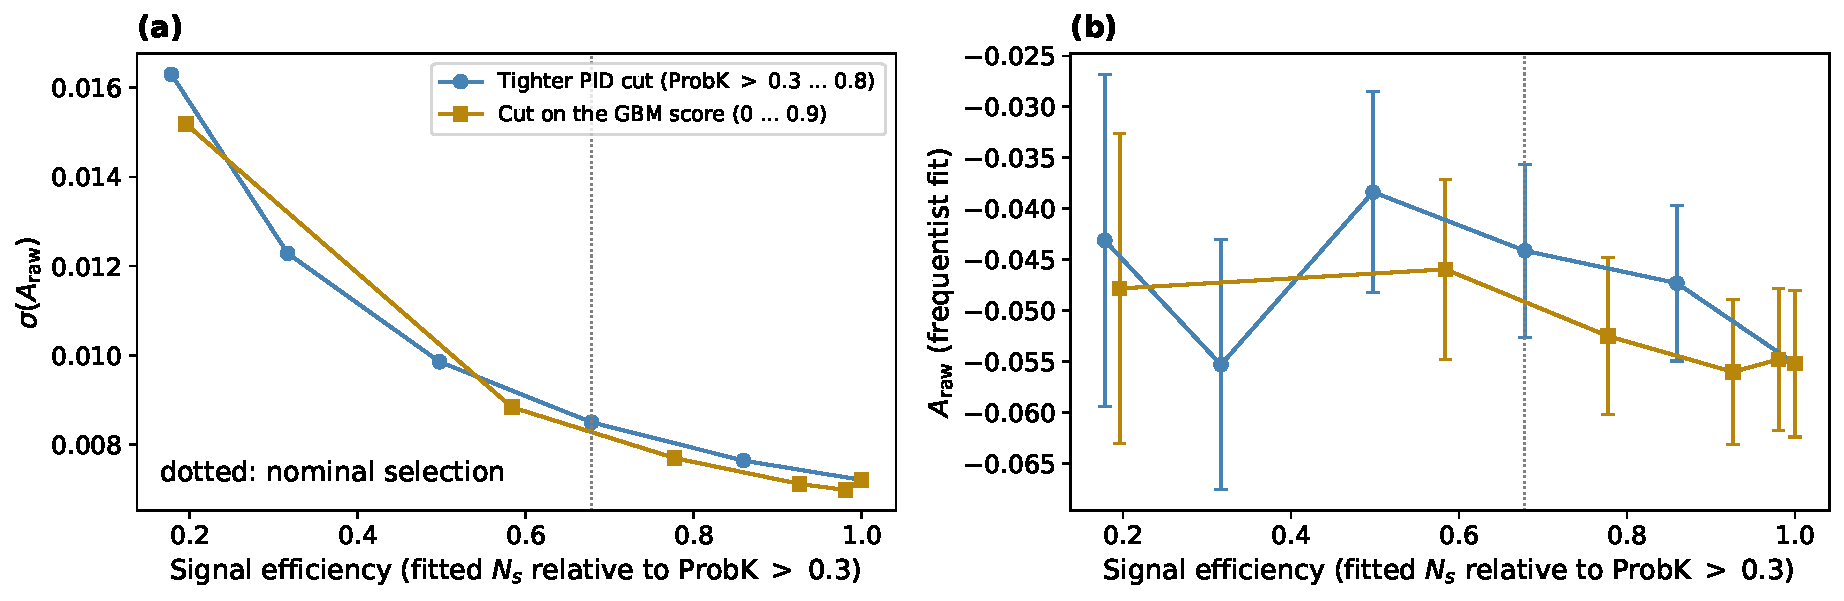
\includegraphics[width=0.95\textwidth]{figures/ml_nominal_high_background.pdf}
\caption{High-background sample ($\texttt{ProbK}>0.3$): (a) statistical uncertainty and (b) value of $\Araw$ from the frequentist fit vs signal efficiency, for tighter identification cuts ($\texttt{ProbK}>0.3,\dots,0.8$) and for cuts on the score of the classifier retrained on this sample ($0,\dots,0.9$). The dotted line marks the nominal selection ($\texttt{ProbK}>0.5$). The samples are nested, so their uncertainties are correlated.}
\label{fig:ml_high_bkg}
\end{figure*}
\clearpage
\subsection{Floats Cited in the Main Text}
The main text cites Fig.~\ref{fig:ml_threshold}, Fig.~\ref{fig:ml_mass_cut}; they are placed here to keep the main text within its page limit.

\begin{figure}[h]
\centering
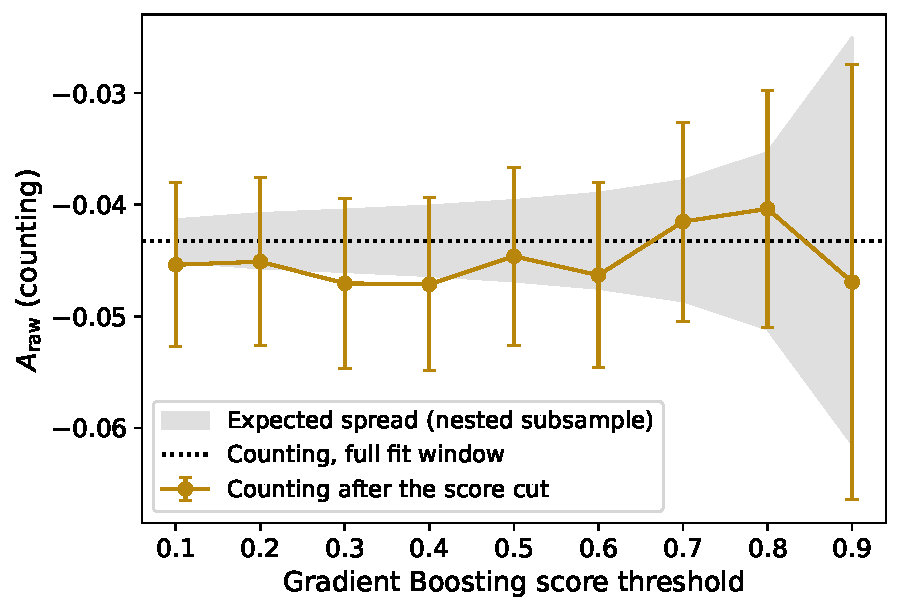
\includegraphics[width=\columnwidth]{figures/ml_nominal_threshold.pdf}
\caption{Counting asymmetry after a cut on the gradient-boosting score, vs.\ threshold, with its binomial uncertainty. Dotted line: counting asymmetry of the full fit window; band: expected statistical spread of a nested subsample around it, $\pm\sqrt{\sigma_{\mathrm{sub}}^2-\sigma_{\mathrm{full}}^2}$.}
\label{fig:ml_threshold}
\end{figure}

\begin{figure*}[t]
\centering
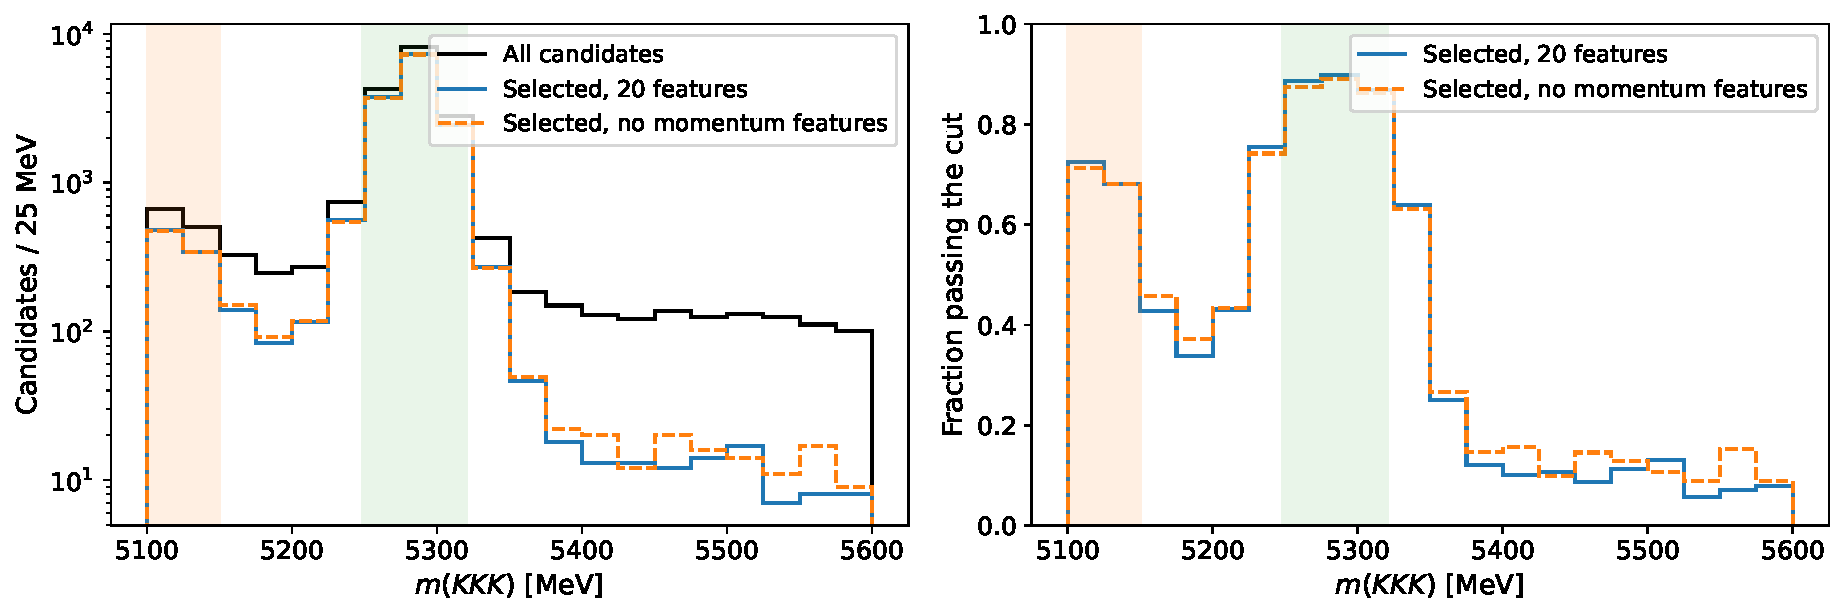
\includegraphics[width=0.95\textwidth]{figures/ml_nominal_mass_after_cut.pdf}
\caption{(a) Mass spectrum of all candidates and of those with gradient-boosting score $>0.5$, for the 20-feature classifier and for one trained without the kaon momentum components (25\,MeV bins). (b) Fraction of candidates passing the cut. Hatched: the region below $5150\,\MeV$ excluded from the background-like labels; grey: the signal-like window.}
\label{fig:ml_mass_cut}
\end{figure*}


\FloatBarrier


\section{Extended Comparison}
\label{app:ext_comp}
\subsection{Numerical Agreement}
\label{sec:comparison_numbers}
The two fits of the same model agree to the precision of the quoted digits: the estimates differ by $0.0002$ ($0.02$ standard deviations), the uncertainties are both $0.0085$, the $68\%$ and $95\%$ intervals differ by at most $0.0002$, and the shifts of the thirteen systematic variants agree within $0.0005$, with the same group uncertainties for the window ($0.0014$) and the preselection ($0.0058$) and slightly different ones for the background ($0.0037$ against $0.0040$) and the signal model ($0.0002$ against $0.0006$), so that the total systematic uncertainties are $0.0070$ and $0.0072$ (Sec.~\ref{sec:syst}). A third estimate, by sideband subtraction (counting in the signal region after removing the background expected from the sideband fit), gives $-0.0503\pm0.0083$, which differs from the nominal value by $0.006$, less than one standard deviation, on the same candidates. This is expected, and it is not by itself a validation of the model. With $\sim2\times10^4$ candidates and flat priors the posterior is proportional to the likelihood, the likelihood is close to a Gaussian in $A$, and the posterior mode coincides with the maximum-likelihood estimate; the posterior median, the posterior mean and the mode differ by less than $2\times10^{-4}$. What the agreement does show is that neither the sampling (MCMC) nor the asymptotic approximations (Hesse, Wilks) introduce a bias: the Bayesian intervals have the coverage of the frequentist ones (Sec.~\ref{sec:bayes_toymc}) and the profile-likelihood interval has the coverage assumed by Wilks' theorem (Sec.~\ref{sec:freq_coverage}).

The agreement does not extend to the validity of the model itself. Both methods describe the same spectrum with the same Gaussian signal and double-exponential background, and neither reaches $\chi^2/\mathrm{ndof}\approx1$ (Sec.~\ref{sec:bayes_gof}); what protects $\Araw$ is that its value does not depend on the signal shape (shift $-0.0002$ with a Crystal Ball) and that the background treatment, the largest model dependence, is included in the systematic uncertainty.

\subsection{Machine Learning and the Fits}
\label{sec:comparison_ml}
The machine-learning selection was used as a cross-check of the fits, not as a replacement. A cut on the gradient-boosting score at $0.5$ keeps $92\%$ of the fitted signal and $36\%$ of the background and does not change $\Araw$ beyond its expected statistical spread, with both inference methods ($-0.0451\pm0.0087$ Bayesian, $-0.0447\pm0.0086$ frequentist, against $-0.0443$ and $-0.0441$ for the full window). It does not improve the precision, $0.0087$ against $0.0085$, because the nominal sample contains little background. In a sample with a looser kaon identification ($33{,}328$ candidates) the classifier raises the purity from $94\%$ to $99\%$ and reduces $\sigma(\Araw)$ from $0.0072$ to $0.0070$ at best, and it cannot remove the misidentified decays that move $\Araw$ to $-0.055$: they peak under the signal, and weak labels derived from the mass spectrum mark them as signal-like (Sec.~\ref{sec:ml_stability}). The useful role of the machine-learning module is therefore that of a consistency test of the asymmetry under a different event selection, and the partition of the Dalitz plane that it provides (below). Gaining precision or controlling the peaking background would require labels that carry information beyond the mass, such as simulation.

\subsection{Bayesian and Frequentist Intervals at Low Statistics}
\label{sec:bayes_lowstat}
\emph{In short: credible and confidence intervals coincide for $\sim2\times10^4$ candidates with flat priors, and stay equal, in value and coverage, down to $50$ candidates.}
With $\sim$$2\times10^4$ candidates the posterior is Gaussian and, with flat priors, the Bayesian and frequentist results coincide by construction (Sec.~\ref{sec:bayes_posterior}). To find where they could differ, the same likelihood was analysed with both methods on toy-MC datasets of $N=50$, $150$, $500$ and $2000$ candidates, $300$ for each size. The model is the six-parameter one of Sec.~\ref{sec:bayes_minimal} (Gaussian signal, one exponential background shared by the charges), which stays identifiable down to a few tens of events; the parameters are those of its fit to the data, with the yields rescaled. Each replica is analysed with the MCMC (median and equal-tailed credible intervals) and by maximum likelihood with \texttt{iminuit} (Hesse intervals, and Minos intervals from the profile likelihood and Wilks' theorem).

\begin{figure*}[t]
\centering
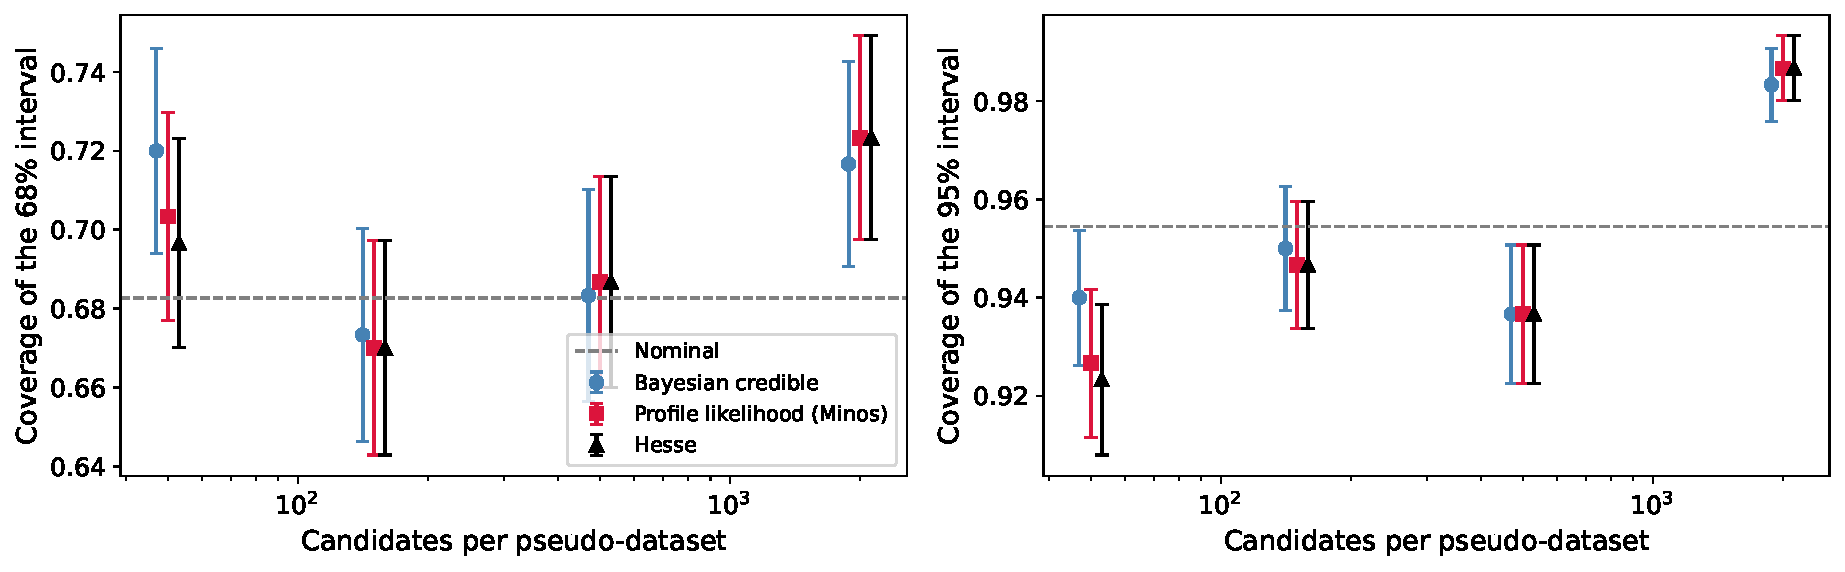
\includegraphics[width=0.95\textwidth]{figures/bayes_nominal_lowstat.pdf}
\caption{Coverage of the (a) 68\% and (b) 95\% intervals on $A$ vs the number of candidates, for the Bayesian credible interval, the profile-likelihood (Minos) interval and the Hesse interval of the same likelihood; 300 toy-MC datasets per point, binomial uncertainties. The dashed lines mark the nominal coverage ($1\sigma$, $2\sigma$; the Bayesian 95\% interval is the 2.5--97.5\% one).}
\label{fig:bayes_lowstat}
\end{figure*}

The two methods agree at every size (Fig.~\ref{fig:bayes_lowstat}). The coverages of the three intervals are compatible with nominal and with each other, the posterior median and the maximum-likelihood estimate differ on average by $5\%$ of the statistical uncertainty at $N=50$ and by less above, and the credible intervals stay symmetric (at $N=50$ the shortest chain is only $\approx10$ autocorrelation times long, so the Monte Carlo error on the interval endpoints is larger there). The asymmetry is a ratio of Poisson yields, whose likelihood is close to Gaussian already with a few tens of signal events: in this problem flat-prior credible intervals and profile-likelihood confidence intervals give the same answer, and Wilks' theorem holds, down to $N=50$. The two approaches differ in what the interval means and in hypothesis testing (Sec.~\ref{sec:bayes_factor}), not in the numbers. At $N=2000$ all three intervals over-cover slightly ($0.98$--$0.99$ for the 95\% interval); since the effect is the same for the three methods, it is a feature of this set of replicas rather than of either inference.

\FloatBarrier
